\chapter{Tools} \label{chap:tools}

This chapter presents the tools that were used to show the feasibility of the
prototype implemented during the course og this work. These tools include
JiST/SWANS discrete event simulator and Sun Small Programable Object
Technology (Sun SPOT) hardware platform. 

\section {JiST/SWANS simulator} \label{sec:jistswans}

As the simulator used in this work is a discrete event simulator, this section
begins with a short description of discrete event simulators. This is followed by
a discussion on the SWANS network simulator used during the course of this work,
and the JiST Java-based discrete event simulator upon which SWANS is built.

\subsection{Discrete Event Simulator}

A discrete event simulator allows for the simulated execution of a process (that
may be either deterministic or stochastic), and consists of the following
components \cite{Shankar_DiscreteEventSim}:

\begin{itemize}
  \item \emph{Simulation variables:} These variables keep track of simulation 
  time, the list of events to be simulated, the (evolving) system state, and 
  performance indicators.
  \item \emph{Event handler:} The event handler schedules events for execution 
  at specific points in simulation time (and unschedules them if necessary), 
  and additionally updates the state variables and performance indicators.
\end{itemize}
 
\subsection{Java In Simulation Time (JiST)} \label{subsec:jist}

JiST \cite{barr_JIST:2005} is a discrete event simulator that is 
efficient (compared to existing simulation systems), 
transparent (simulations are automatically translated to run with the 
simulation time semantics), and standard (simulations use a
conventional programming language, i.e., Java).

JiST simulation code is written in Java, and converted to run over the JiST 
simulation kernel using a bytecode-level rewriter\footnote{The bytecode 
rewriter and the simulation kernel are both written in Java},  as can be
seen in Figure \ref{Fig:JiST_architecture}.

The execution of a JiST program can be understood by considering the example 
shown in Listing \ref{listing:JiSTExample}

\begin{lstlisting}[frame=trbl, basewidth={0.55em, 0.6em}, captionpos=b, 
basicstyle=\ttfamily\footnotesize, breaklines, caption = Example JiST program (reproduced from \cite{barr_JIST:2005}, label = listing:JiSTExample]  
import jist.runtime.JistAPI;  
class hello implements JistAPI.Entity { 
  public static void main(String[] args) { 
    System.out.println("Simulation start"); 
    hello h = new hello(); 
    h.myEvent(); 
  } 
  public void myEvent() { 
    JistAPI.sleep(1); 
    myEvent(); 
    System.out.println("hello world, " + JistAPI.getTime()); 
  }} 
\end{lstlisting}

\begin{figure}
\centering
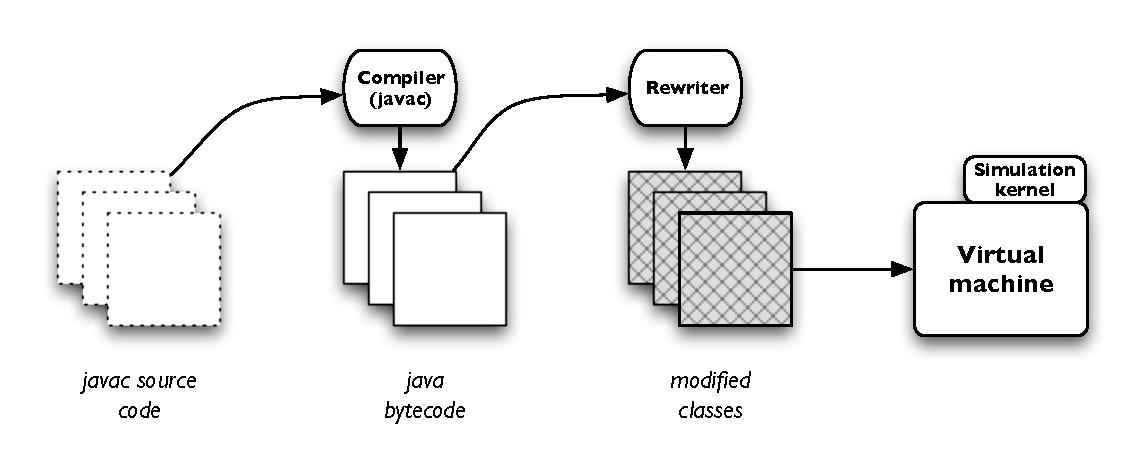
\includegraphics[width=\textwidth]{img/JiST_architecture.eps} 
\caption[The JiST System Architecture]{The JiST system architecture (reproduced from
\cite{barr_JIST:2005})}
\label{Fig:JiST_architecture}
\end{figure}  
 
This program is then compiled and executed in the JiST simulation
kernel, using the following commands:

  
\begin{lstlisting}[frame=trbl, basewidth={0.55em, 0.6em}, captionpos=b, 
basicstyle=\ttfamily\footnotesize, breaklines, caption = Execution of the
program in the JiST, label = listing:JiST ]  
javac hello.java
java jist.runtime.Main hello
\end{lstlisting}


The simulation kernel is loaded upon execution of this command. This kernel
installs into the JVM a class loader that performs the rewrite of the bytecode.
The JiST API functions used in the example code are used to perform the
code transformations. The method call to myEvent is now scheduled and executed
by the simulator in simulation time. Simulation time differs from ``actual''
time in that the advancement of actual time is independent of application
execution, whereas simulation time is not. 
 
\subsection{Scalable Wireless Ad hoc Network Simulator (SWANS)}
SWANS is a wireless network simulator developed in order to provide efficient
and scalable simulations without compromising on simulation detail \cite{barr_SWANS},
and is built upon the JiST discrete event simulator described in Section \ref{subsec:jist}. 
It is organised a a collection of independent, relatively simple, event driven
components that are encapsulated as JiST entities. 

\begin{figure}[h]
\centering
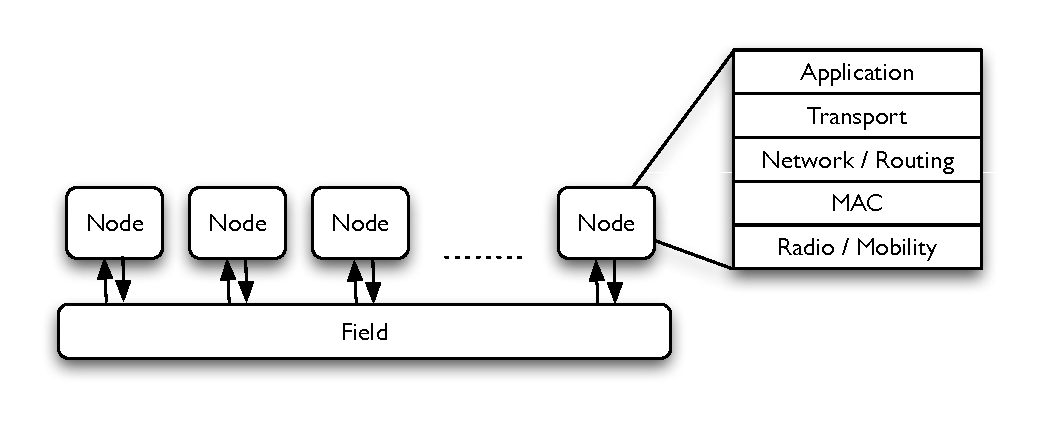
\includegraphics[width=\textwidth]{img/SWANS_architecture.eps} 
\caption[SWANS architecture]{SWANS architecture}
\label{Fig:SWANS_architecture}
\end{figure} 
  
SWANS has the following capabilities \cite{barr_SWANS}:

\begin{itemize}
\item The use of
interchangeable components enables the construction of a protocol stack for the
network, and facilitates parallelism, and execution in a distributed environment.
\item Can execute unmodified Java network applications on the
simulated network (in simulation time), by virtue of its being built over
JiST. Using a harness, the aforementioned Java code is automatically rewritten to
run on the simulated network.  
\end{itemize}
   
The SWANS architecture may be seen in Figure \ref{Fig:SWANS_architecture}. 

\section {Sun SPOT platform} \label{sec:sunspots}

Sensor nodes, as mentioned in Section \ref{subsec:sensornodes}, are
characterised by limited resources, including memory. 

In order to overcome memory limitations, wireless sensor network applications
have traditionally been coded in non-managed languages like C and assembly
language \cite{simon_squawk:2006}.
 
Managed runtime languages like Java were not used for sensor network programming
because of the combination of the static memory footprint of the Java Virtual
Machine (JVM) and the dynamic memory footprint of the WSN application code.
 
On the other hand, it is widely accepted that development times are greatly reduced
upon the use of managed runtime languages such as Java
\cite{simon_squawk:2006}. Therefore, currently prevalent WSN programming practice
trades developer efficiency for memory efficiency. 

However, Simon et al \cite{simon_squawk:2006} state the benefits resulted from
using a managed runtime language for WSN programming as follows:

\begin{itemize}
  \item Simplification of the process of WSN programming, that would cause an
  increase in developer adoption rates and productivity.
  \item Opportunity to use standard development and debugging tools.
\end{itemize}

The use of the Java programming language in SunSPOTs makes it particularly
suitable as a platform for the DADT applications presented. This is because the
DADT programming abstraction is designed to reduce programmer workload, and the
use of a managed runtime language such as Java has been shown to further
improve developer efficiency.
 
Sun Microsystems has, on the basis of the arguments discussed in the previous
section, proposed and built a sensor device
called the Sun Small Programmable Object Technology (Sun SPOT) that uses a
on-board JVM to allow for WSN programming using Java.

The Sun SPOT (see Figure \ref{Fig:SunSpot}) uses an ARM-9 processor, has 512 KB of RAM
and 4 MB of flash memory, uses a 2.4GHz radio with an integrated antenna on the board. The radio
is a TI CC2420 and is IEEE 802.15.4 compliant.

\begin{figure} 
\centering
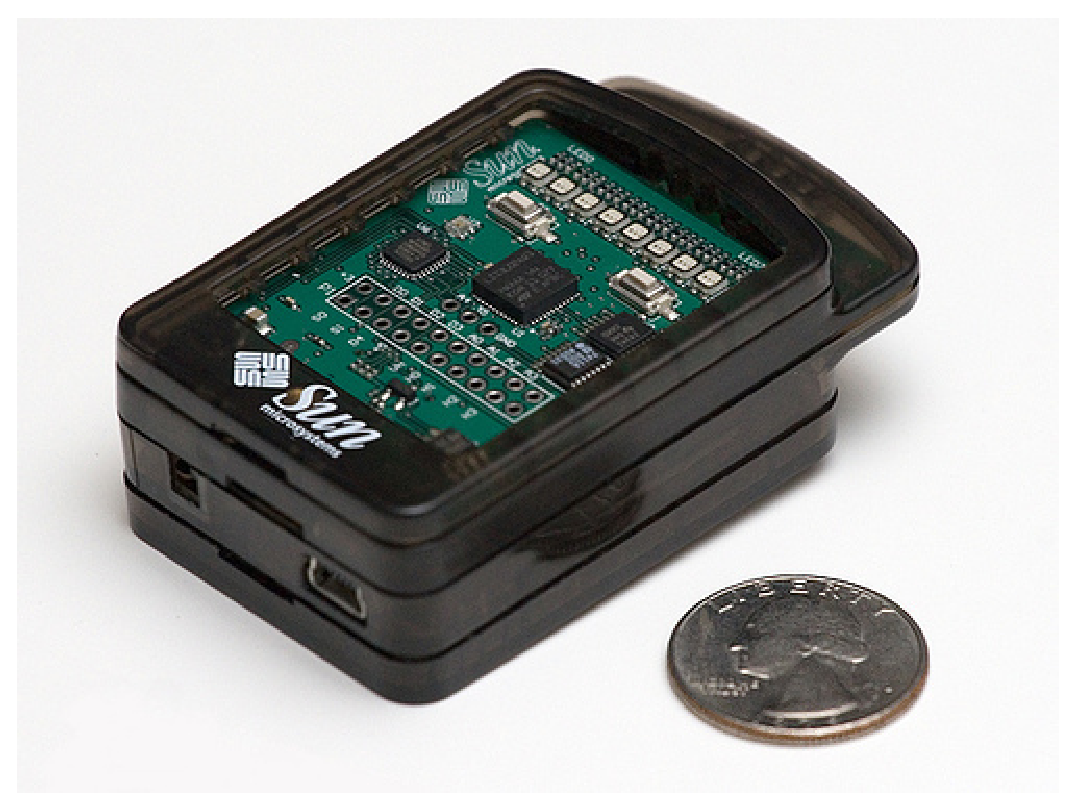
\includegraphics[scale=0.50]{img/sunspot1.eps} 
\caption[Sun SPOT device]{Sun SPOT device}
\label{Fig:SunSpot}
\end{figure} 


\subsection{The Squawk JVM}

The Squawk JVM is used on Sun SPOTs to enable on-board execution of Java
programs. The Squawk VM was originally developed for a smart card system with
even greater memory constraints than the Sun SPOTs. The Squawk JVM has the
following features \cite{simon_squawk:2006}:

\begin{itemize}
  \item It is written in Java, and specifically designed for resource
  constrained devices, meeting the requirements of Connected Limited Device
  Configuration 1.1 (CLDC) framework for Java Micro Edition (Java ME)
  applications.
  \item It does not require an underlying OS as it runs directly on the Sun
  SPOT hardware. This allows for a reduction in memory consumption.
  \item It suuports inter-device application migration.
  \item It allows the execution of multiple applications on one VM,
  representing each one as an object.
\end{itemize}

As resource constrained devices are incapable of loading class files on-device
by virtue of their limited memory, a VM architecture known as the ``split VM
architecture'' is used, as shown in Figure
\ref{Fig:SquawkVM_architecture}.

\begin{figure}[h]
\centering
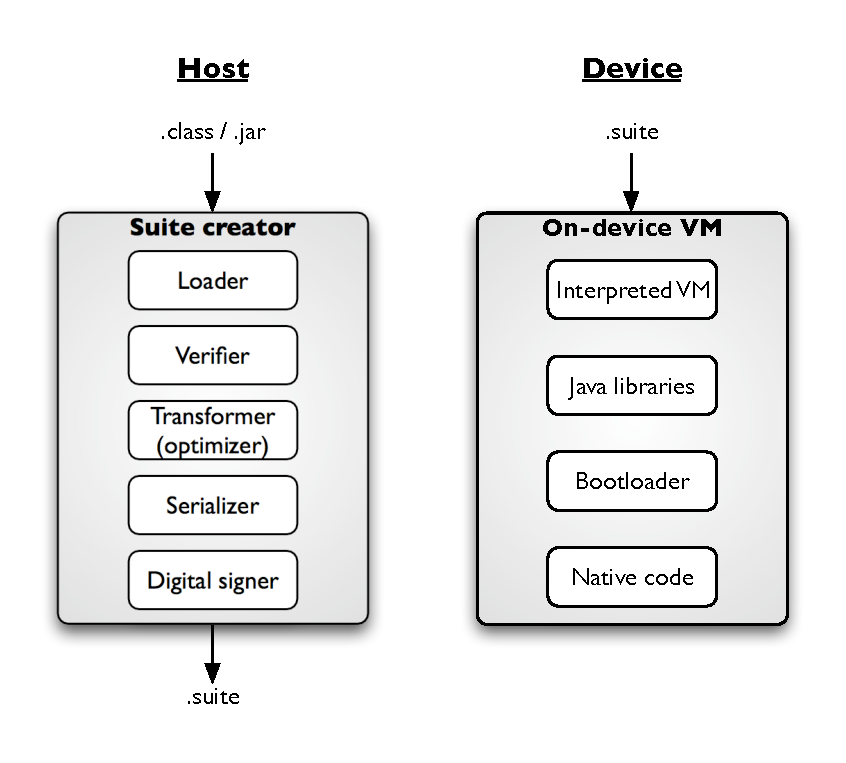
\includegraphics[scale=0.61]{img/Squawk_architecture.eps} 
\caption[The Squawk Split VM Architecture]{The Squawk
Split VM Architecture (reproduced from \cite{simon_squawk:2006})}
\label{Fig:SquawkVM_architecture}
\end{figure}  

The Squawk split VM architecture uses a class file preprocessor known as the
\emph{suite creator} that converts the \emph{.class} bytecode into a more
compact representation called the Squawk bytecode. According to
\cite{simon_squawk:2006}, Squawk bytecodes are optimised in order to:
\begin{itemize}
\item minimise space used by using smaller bytecode representation, escape
mechanisms for float and double instructions, and widened operands. 
\item enable in-place execution, by ``resolving symbolic references to other
classes, data members, and member functions into direct pointers, object offsets
and method table offsets respectively''.
\item simplify garbage collection, by the careful reallocation of local
variables, and by storing on the operand stack the operands of only those instructions that would result in a memory allocation.
\end{itemize}

The Squawk bytecodes are converted into a \emph{.suite} file created by
serialising and saving into a file the internal object memory representation.
These files are loaded on to the device, and subsequently interpreted by the
on-device VM.

\subsection{Sun SPOT applications} \label{subsec:sunspotapps}

Sun SPOT applications are divided into two classes:
\cite{sun_developer:2008}:

\begin{itemize}
  \item \emph{On-SPOT applications}
  \item \emph{On-Host applications}
\end{itemize}

\begin{figure}[h]
\centering
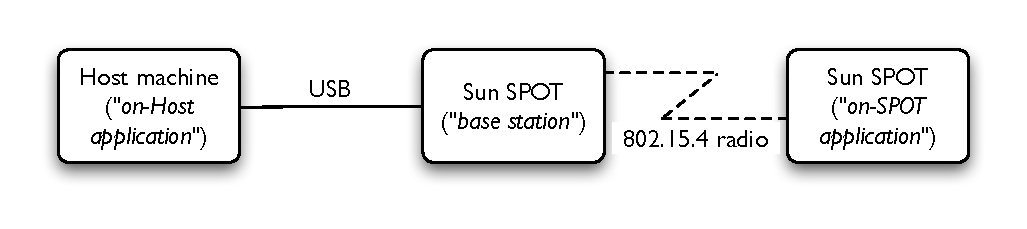
\includegraphics[width=\textwidth]{img/SunSPOTS_applications.eps} 
\caption[Types of Sun SPOT applications]{Types of Sun SPOT applications (adapted from
\cite{sun_developer:2008})}
\label{Fig:SunSPOTS_applications}
\end{figure}  

\emph{On-SPOT applications}  are deployed and
executed on a remote Sun SPOT that communicates untethered. On-SPOT
applications are Java programs that runs on the Squawk VM, and are compliant
with CLDC 1.1 specification. 

\emph{On-Host applications} run on the host machine
(typically a PC), and communicate with the network of Sun SPOTs through a base
station node that serves no purpose other than to facilitate Sun SPOT-host
machine communication. 
  
The base station node, which is a Sun SPOT itself, communicates with other
nodes in the network using RF communication, and with the host machine via a
USB link (see Figure \ref{Fig:SunSPOTS_applications}). The host application is
a Java 2 Standard Edition (J2SE) program.
  
 
\section{Summary}

This chapter presented tools that were used to demonstrate the feasibility of
the prototype implemented as part of this work. The chapter provided an overview of the JIST/SWANS
network simulator used for verification of the prototype. This was followed by
a presentation of the SunSPOTs hardware platform, and its particular suitability for the application under
consideration.


  